%!TEX root = ../rapport.tex
%!TEX encoding = UTF-8 Unicode

% Chapitres "Introduction"

% modifié par Francis Valois, Université Laval
% 31/01/2011 - version 1.0 - Création du document

\chapter{Diagrammes de séquences}
\label{s:sequences}
Ce chapitre présente les différentes figures associées au diagramme des séquences. Ce diagramme est séparé selon cinq portions relatives aux fonctions particulières du robot. La figure \ref{fig:diagSeq1Ite1} présente les liens entre l'utilisateur et la kinocto. La figure \ref{diagSeq2Ite1} présente les liens entre la kinocto et son environnement afin de déterminer sa position ainsi que le décodage de l'antenne avec les mouvements associés pour arriver. La figure \ref{diagSeq3Ite1} présente les liens entre la kinocto et la station de base pour la transmission et l'affichage ainsi que la lecture et le décodage du sudocube avec les mouvements nécessaires pour y arriver. La figure \ref{diagSeq4Ite1} présente les liens entre la kinocto et la table de jeu dans l'optique du déplacement de celui-ci pour effectuer le dessin du chiffre contenu dans la case rouge du sudocube.
\begin{figure}[htb]
\centering
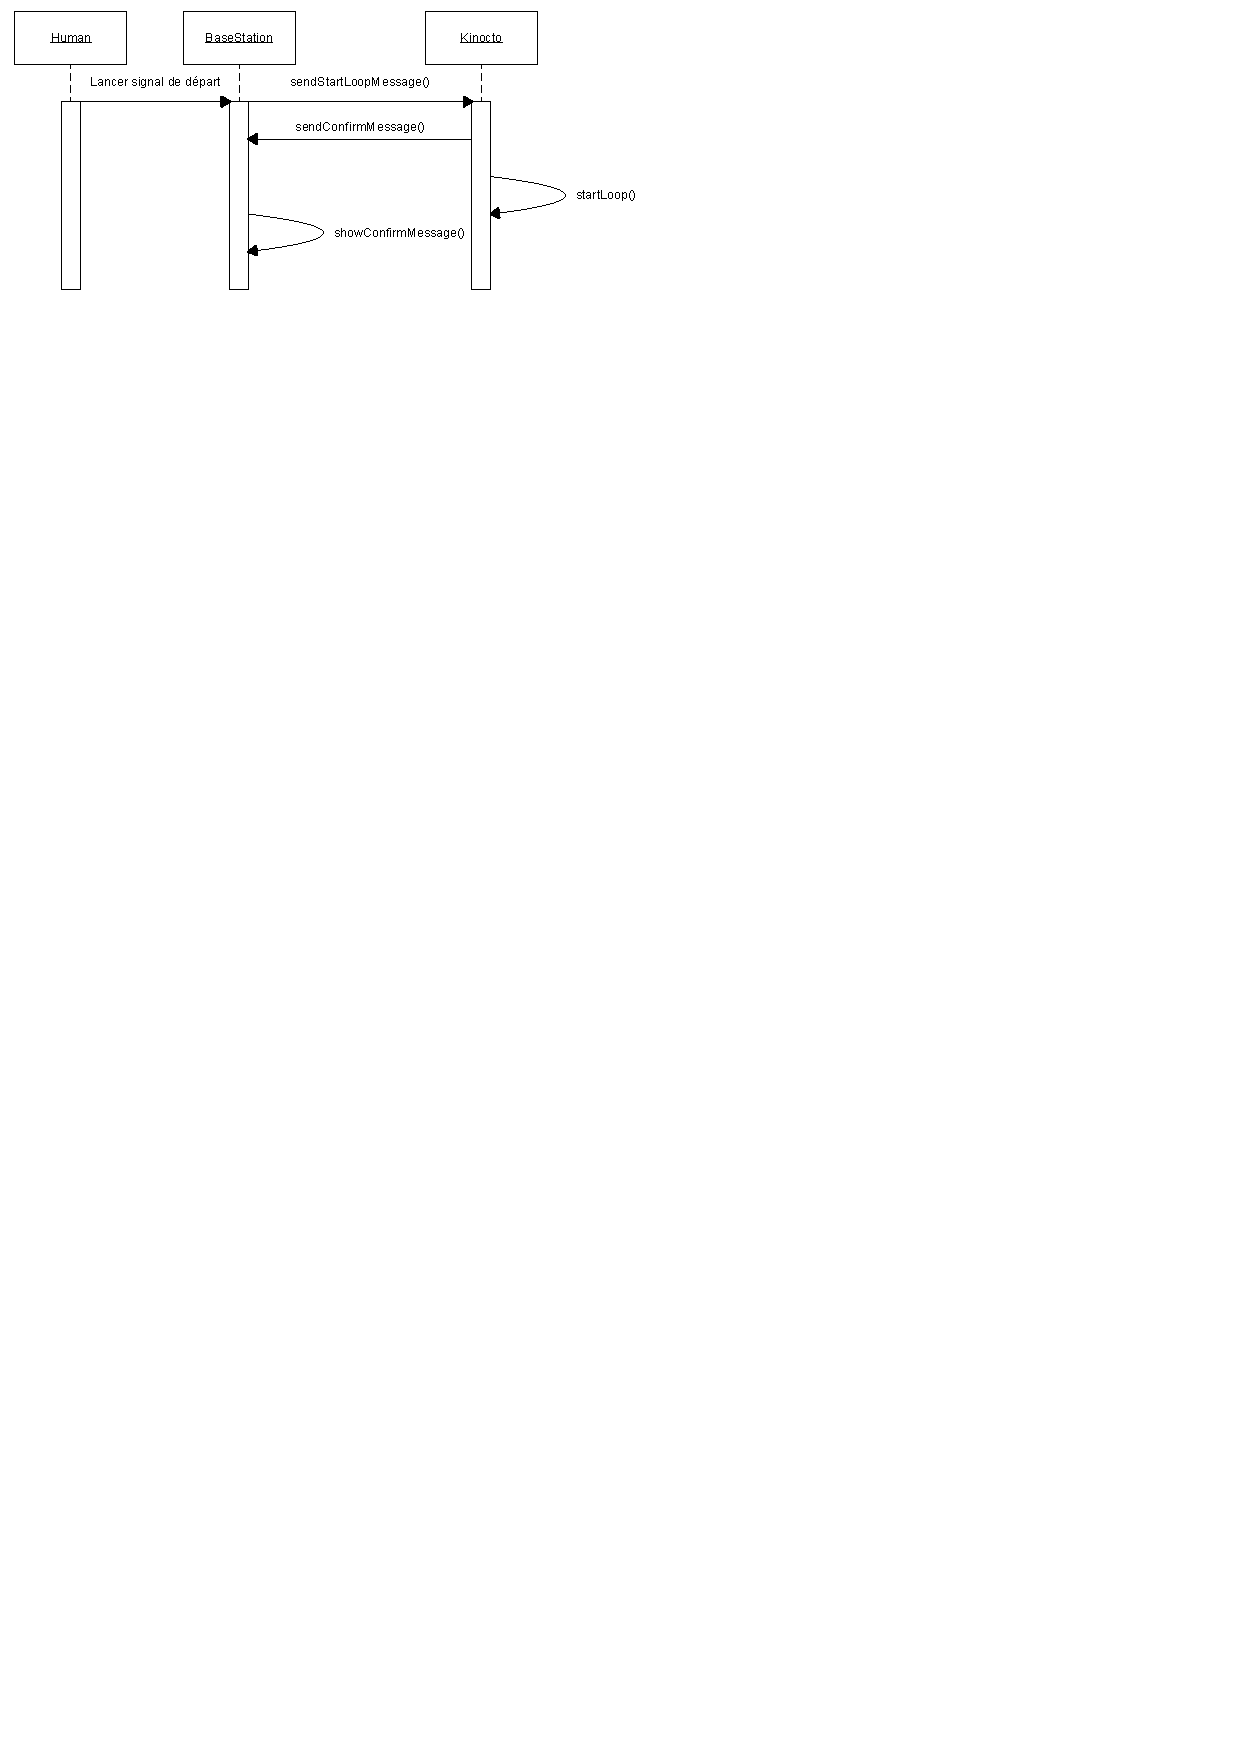
\includegraphics[scale=1]{diagrammes_sequence1.pdf}
\caption{Diagramme des séquences présentant les liens entre l'utilisateur et la kinocto}
\label{fig:diagSeq1Ite1} 
\end{figure}

\begin{landscape}
\begin{figure}[htb]
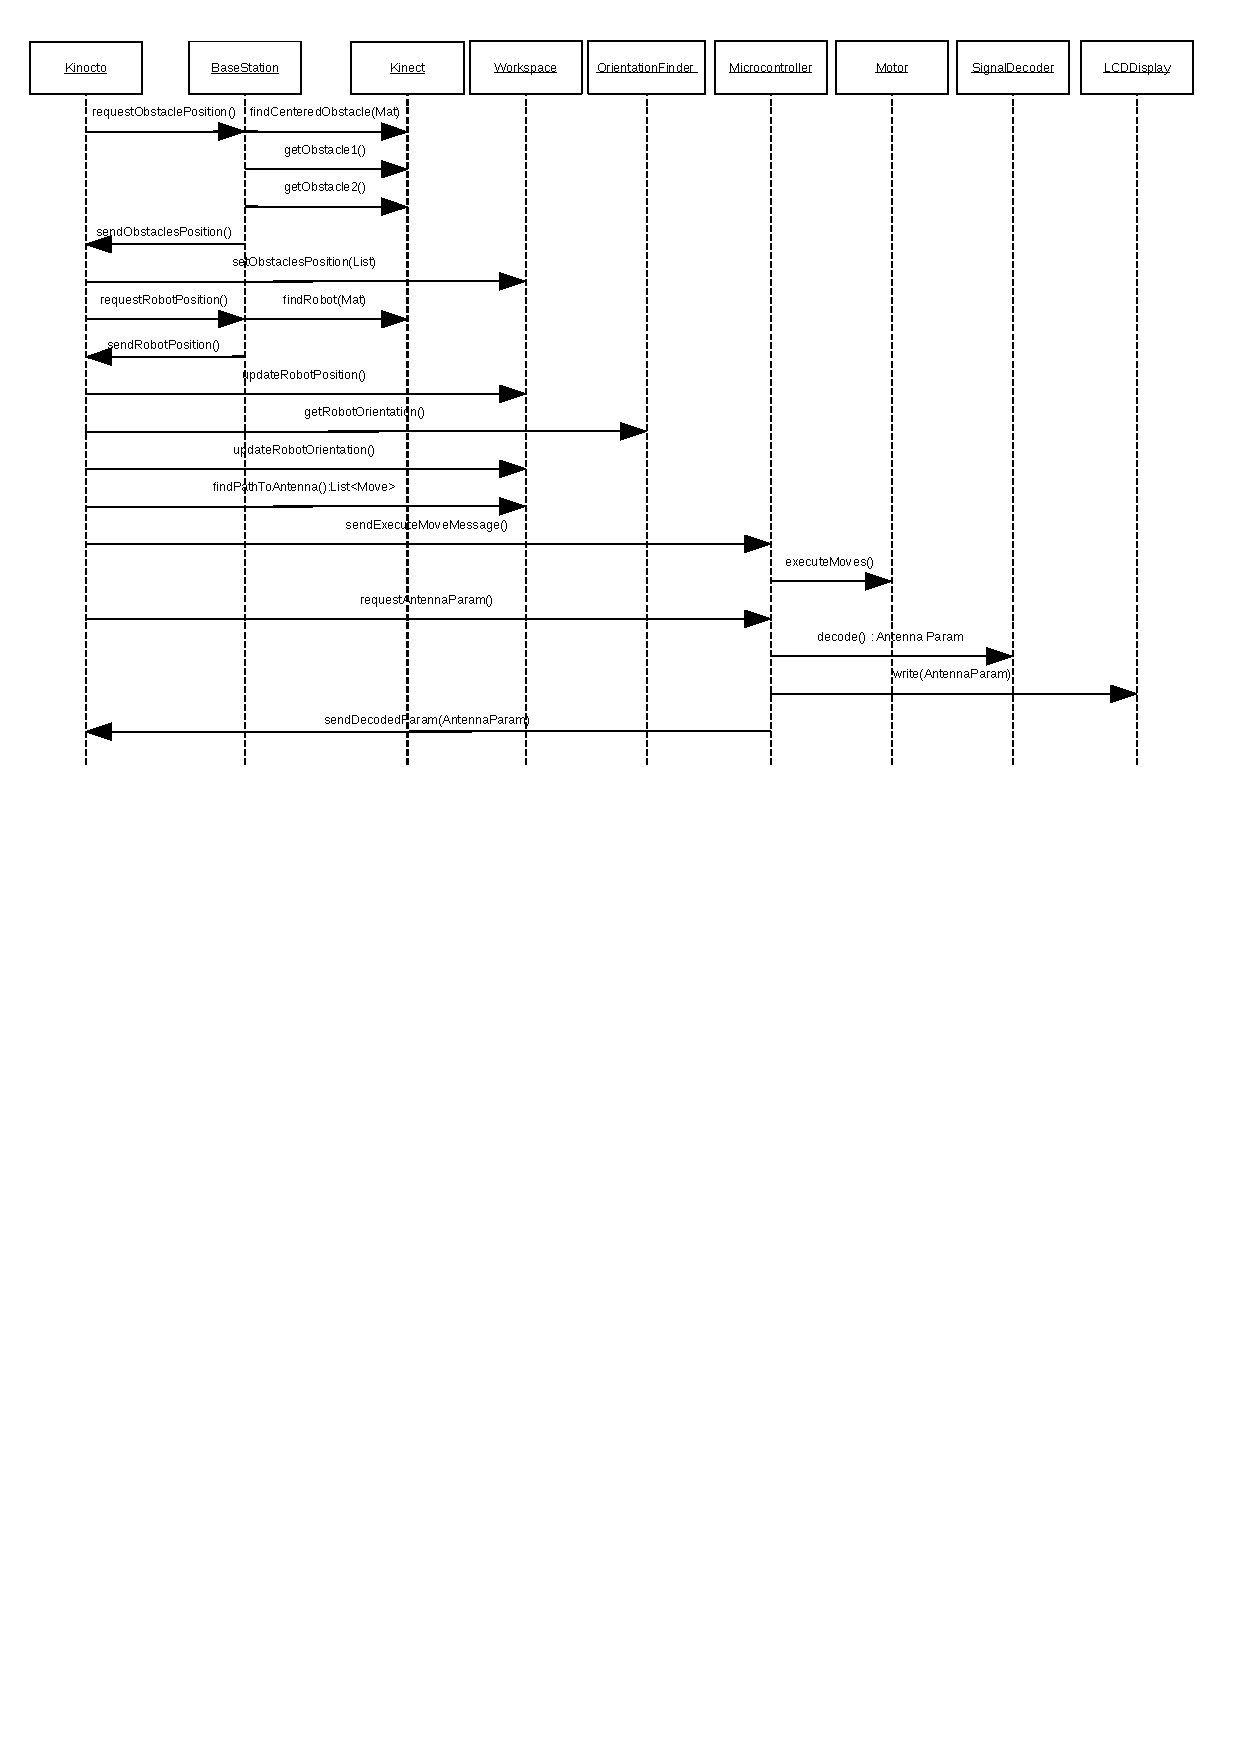
\includegraphics[scale=1]{diagrammes_sequence2.pdf}
\caption{Diagramme des séquences présentant les liens entre la kinocto et son environnement afin de déterminer sa position ainsi que le décodage de l'antenne avec les mouvements associés pour arriver}
\label{diagSeq2Ite1}
\end{figure}

\begin{figure}[htb]
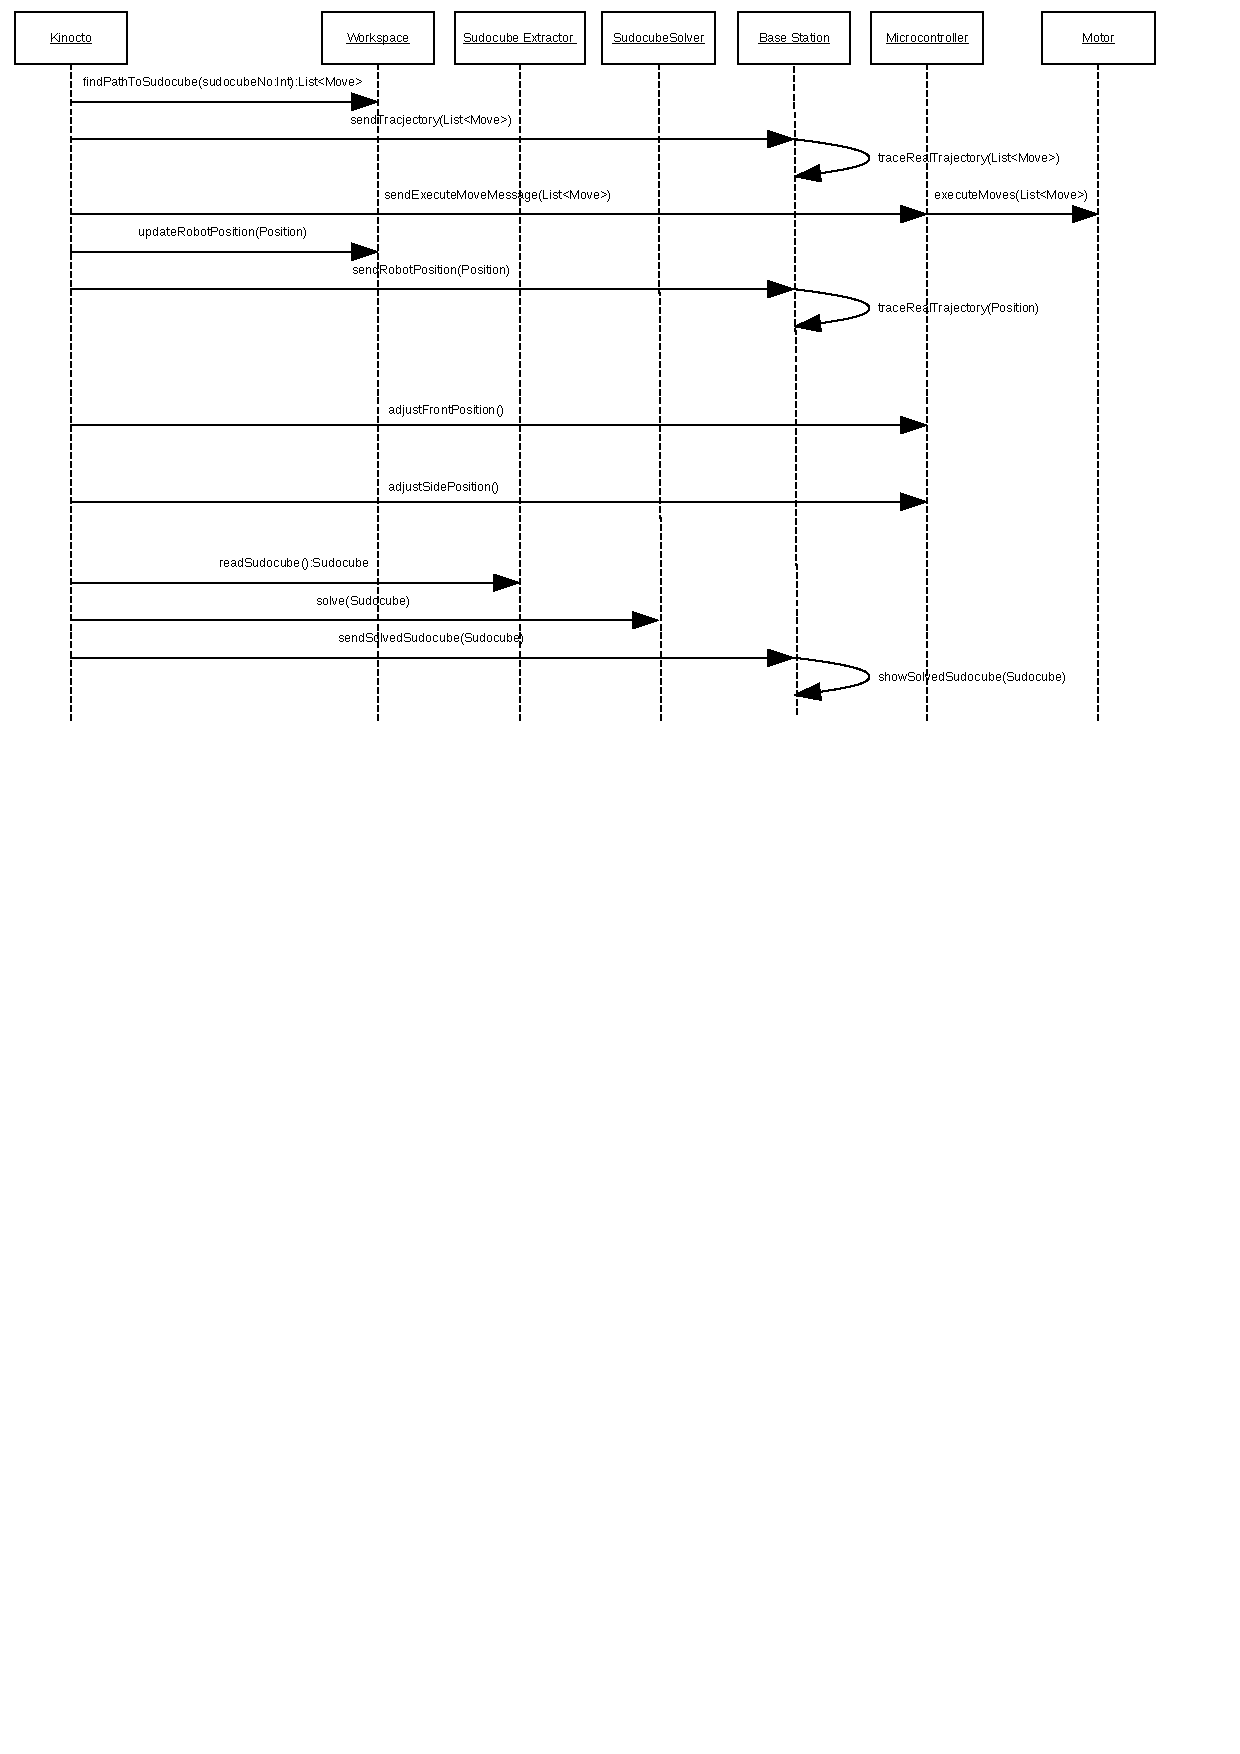
\includegraphics[scale=1]{diagrammes_sequence3.pdf}
\caption{Diagramme des séquences présentant les liens entre la kinocto et la station de base pour la transmission et l'affichage ainsi que la lecture et le décodage du sudocube avec les mouvements nécessaires pour y arriver}
\label{diagSeq3Ite1}
\end{figure}

\begin{figure}[htb]
	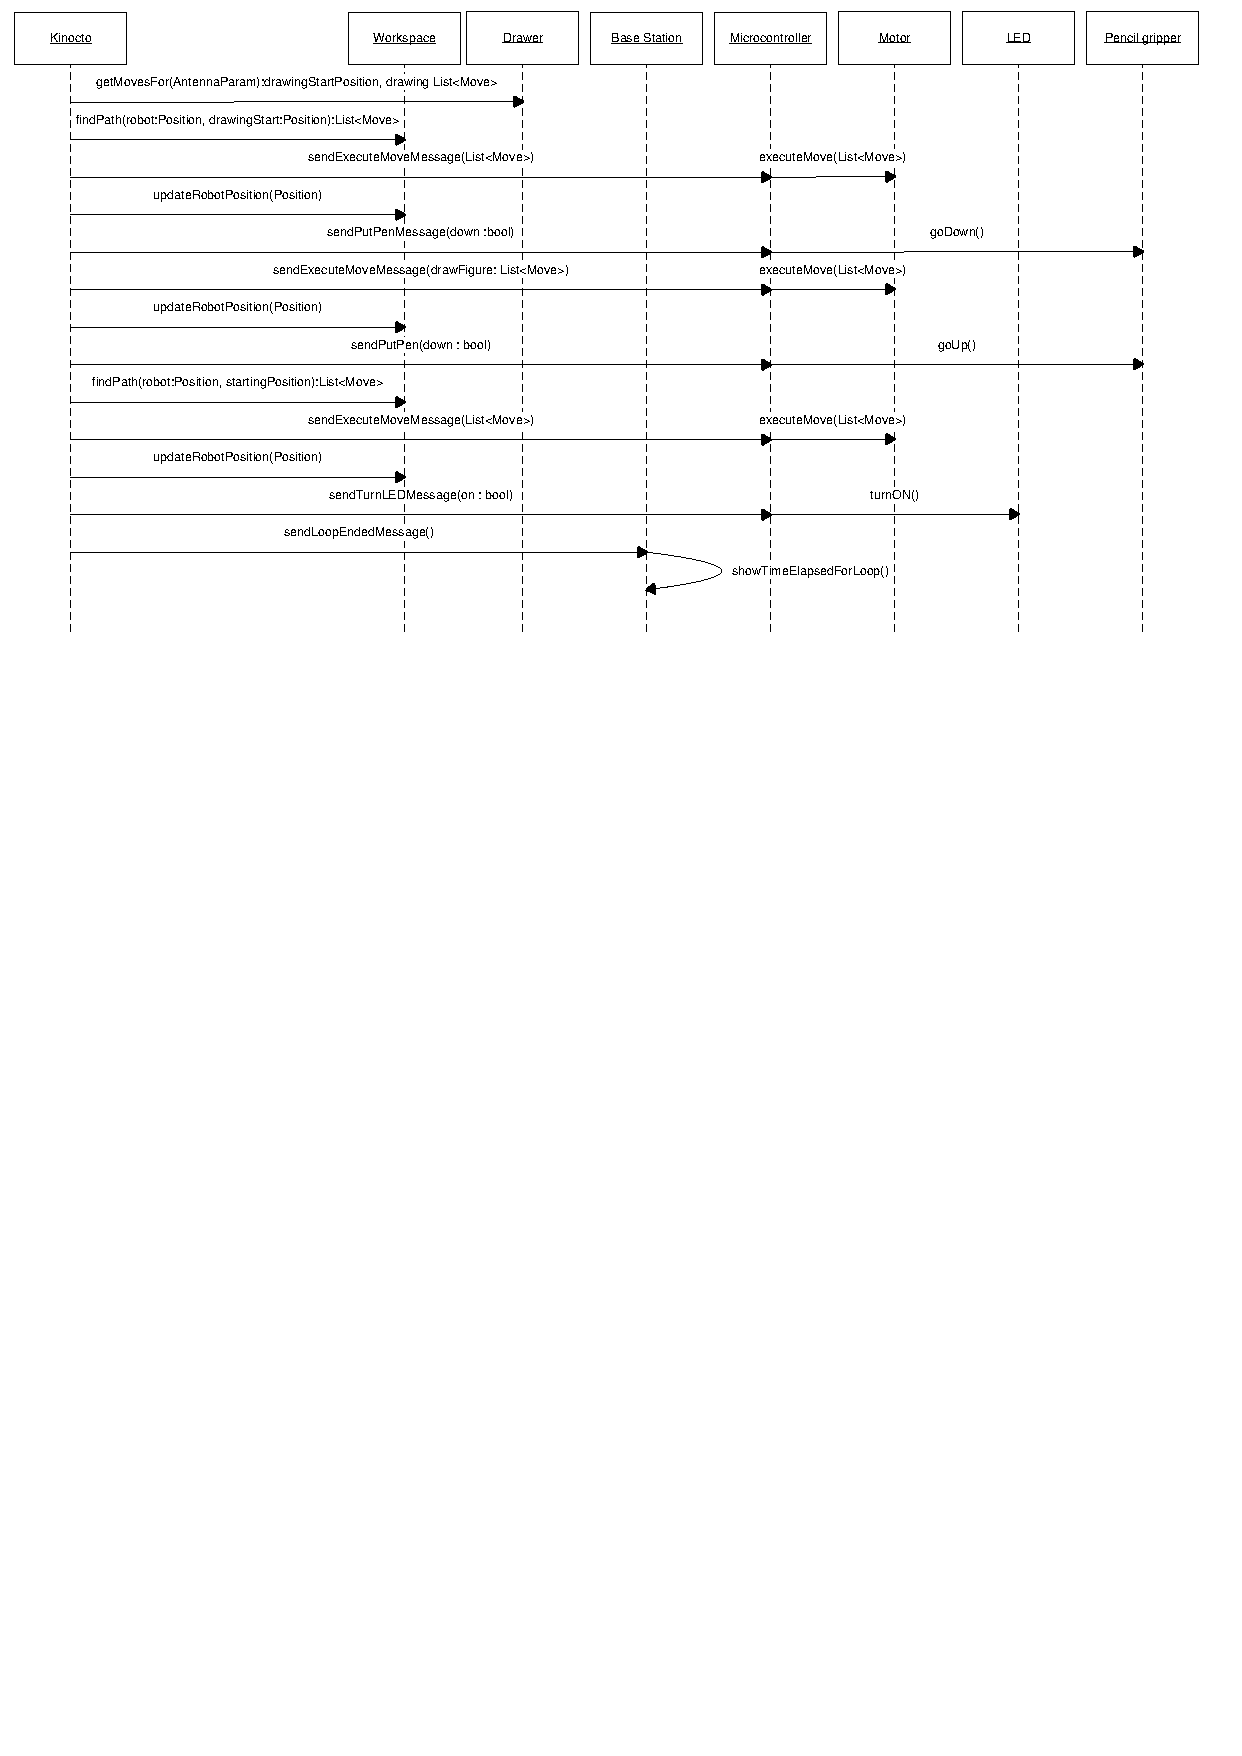
\includegraphics[scale=1]{diagrammes_sequence4.pdf}
\caption{Diagramme des séquences présentant les liens entre la kinocto et la table de jeu dans l'optique du déplacement de celui-ci pour effectuer le dessin du chiffre contenu dans la case rouge du sudocube}
\label{diagSeq4Ite1}
\end{figure}

\end{landscape}
